\section{Limitações, Spearman e Simpson}

\begin{frame}{Propriedades do Coeficiente $r$}
    \begin{itemize}
        \item \textbf{Invariância por Escala e Translação:}
        \begin{itemize}
            \item Somar ou subtrair constantes aos dados não altera $r$.
            \item Multiplicar os dados por uma constante positiva não altera $r$.
            \item $\implies$ a correlação independe das unidades físicas de medida utilizadas.
        \end{itemize}
        \item \textbf{Simetria:} A correlação entre $X$ e $Y$ é idêntica à de $Y$ e $X$ ($r_{XY} = r_{YX}$).
        \item \textbf{Interpretação Geométrica:}
        \begin{itemize}
            \item O $r$ de Pearson equivale ao cosseno do ângulo $\theta$ entre os vetores de desvios normalizados:
            $$r = \cos(\theta)$$
            \item Vetores ortogonais ($\theta = 90^\circ$) possuem correlação nula ($r = 0$).
            \item Vetores na mesma linha ($\theta = 0^\circ$ ou $180^\circ$) possuem correlação perfeita ($r = 1$ ou $-1$).
        \end{itemize}
    \end{itemize}
\end{frame}

\begin{frame}{Armadilhas da Correlação Linear}
    \begin{itemize}
        \item \textbf{Mede apenas Relações Lineares:}
        \begin{itemize}
            \item Se $Y = X^2$ de forma exata, existe uma relação determinística perfeita.
            \item Contudo, o cálculo do $r$ de Pearson para um intervalo simétrico em torno de zero (ex: $[-2, 2]$) resultará em $r = 0$.
        \end{itemize}
        \item \textbf{Alta Sensibilidade a Outliers:}
        \begin{itemize}
            \item Um único valor extremo fora do padrão de dispersão geral dos dados pode inflar artificialmente ou reduzir drasticamente o valor de $r$.
        \end{itemize}
        \item \textbf{Correlações Ecológicas:}
        \begin{itemize}
            \item Tirar conclusões sobre indivíduos com base na correlação de dados agrupados em grandes grupos (ex: média de renda urbana por país vs. taxa de criminalidade).
        \end{itemize}
    \end{itemize}
\end{frame}

\begin{frame}{A Correlação de Postos de Spearman ($r_s$)}
    \begin{itemize}
        \item Quando a relação é não-linear mas ainda preserva uma ordem monotônica (ambas crescem ou decrescem juntas), Pearson falha em medir a intensidade total.
        \item A alternativa é a \textbf{Correlação de Postos de Spearman} ($r_s$):
        \begin{enumerate}
            \item Ordenamos os dados de $X$ e de $Y$ separadamente.
            \item Substituímos cada valor original pelo seu respectivo Posto (ou Posição de ordenação, de $1$ a $N$).
            \item Calculamos o Coeficiente de Pearson sobre estes postos ordinais.
        \end{enumerate}
        \item \textbf{Vantagens:}
        \begin{itemize}
            \item Mede qualquer relação monotônica (curvas não-lineares coerentes).
            \item Muito mais resistente a valores atípicos extremos (outliers).
        \end{itemize}
    \end{itemize}
\end{frame}

\begin{frame}[fragile]{Exemplo Pareado: Pearson vs. Spearman}
    \begin{columns}
        \begin{column}{0.48\textwidth}
            \textbf{Caso Prático:}
            \begin{itemize}
                \item Análise de uma curva exponencial com ruído.
                \item O ajuste linear clássico é pobre para esta tendência acelerada.
                \item \textbf{Resultados:}
                \begin{itemize}
                    \item Pearson $r \approx 0.86$ (subestima a força da associação).
                    \item Spearman $r_s \approx 0.99$ (identifica a relação monotônica quase perfeita).
                \end{itemize}
            \end{itemize}
            \centering
            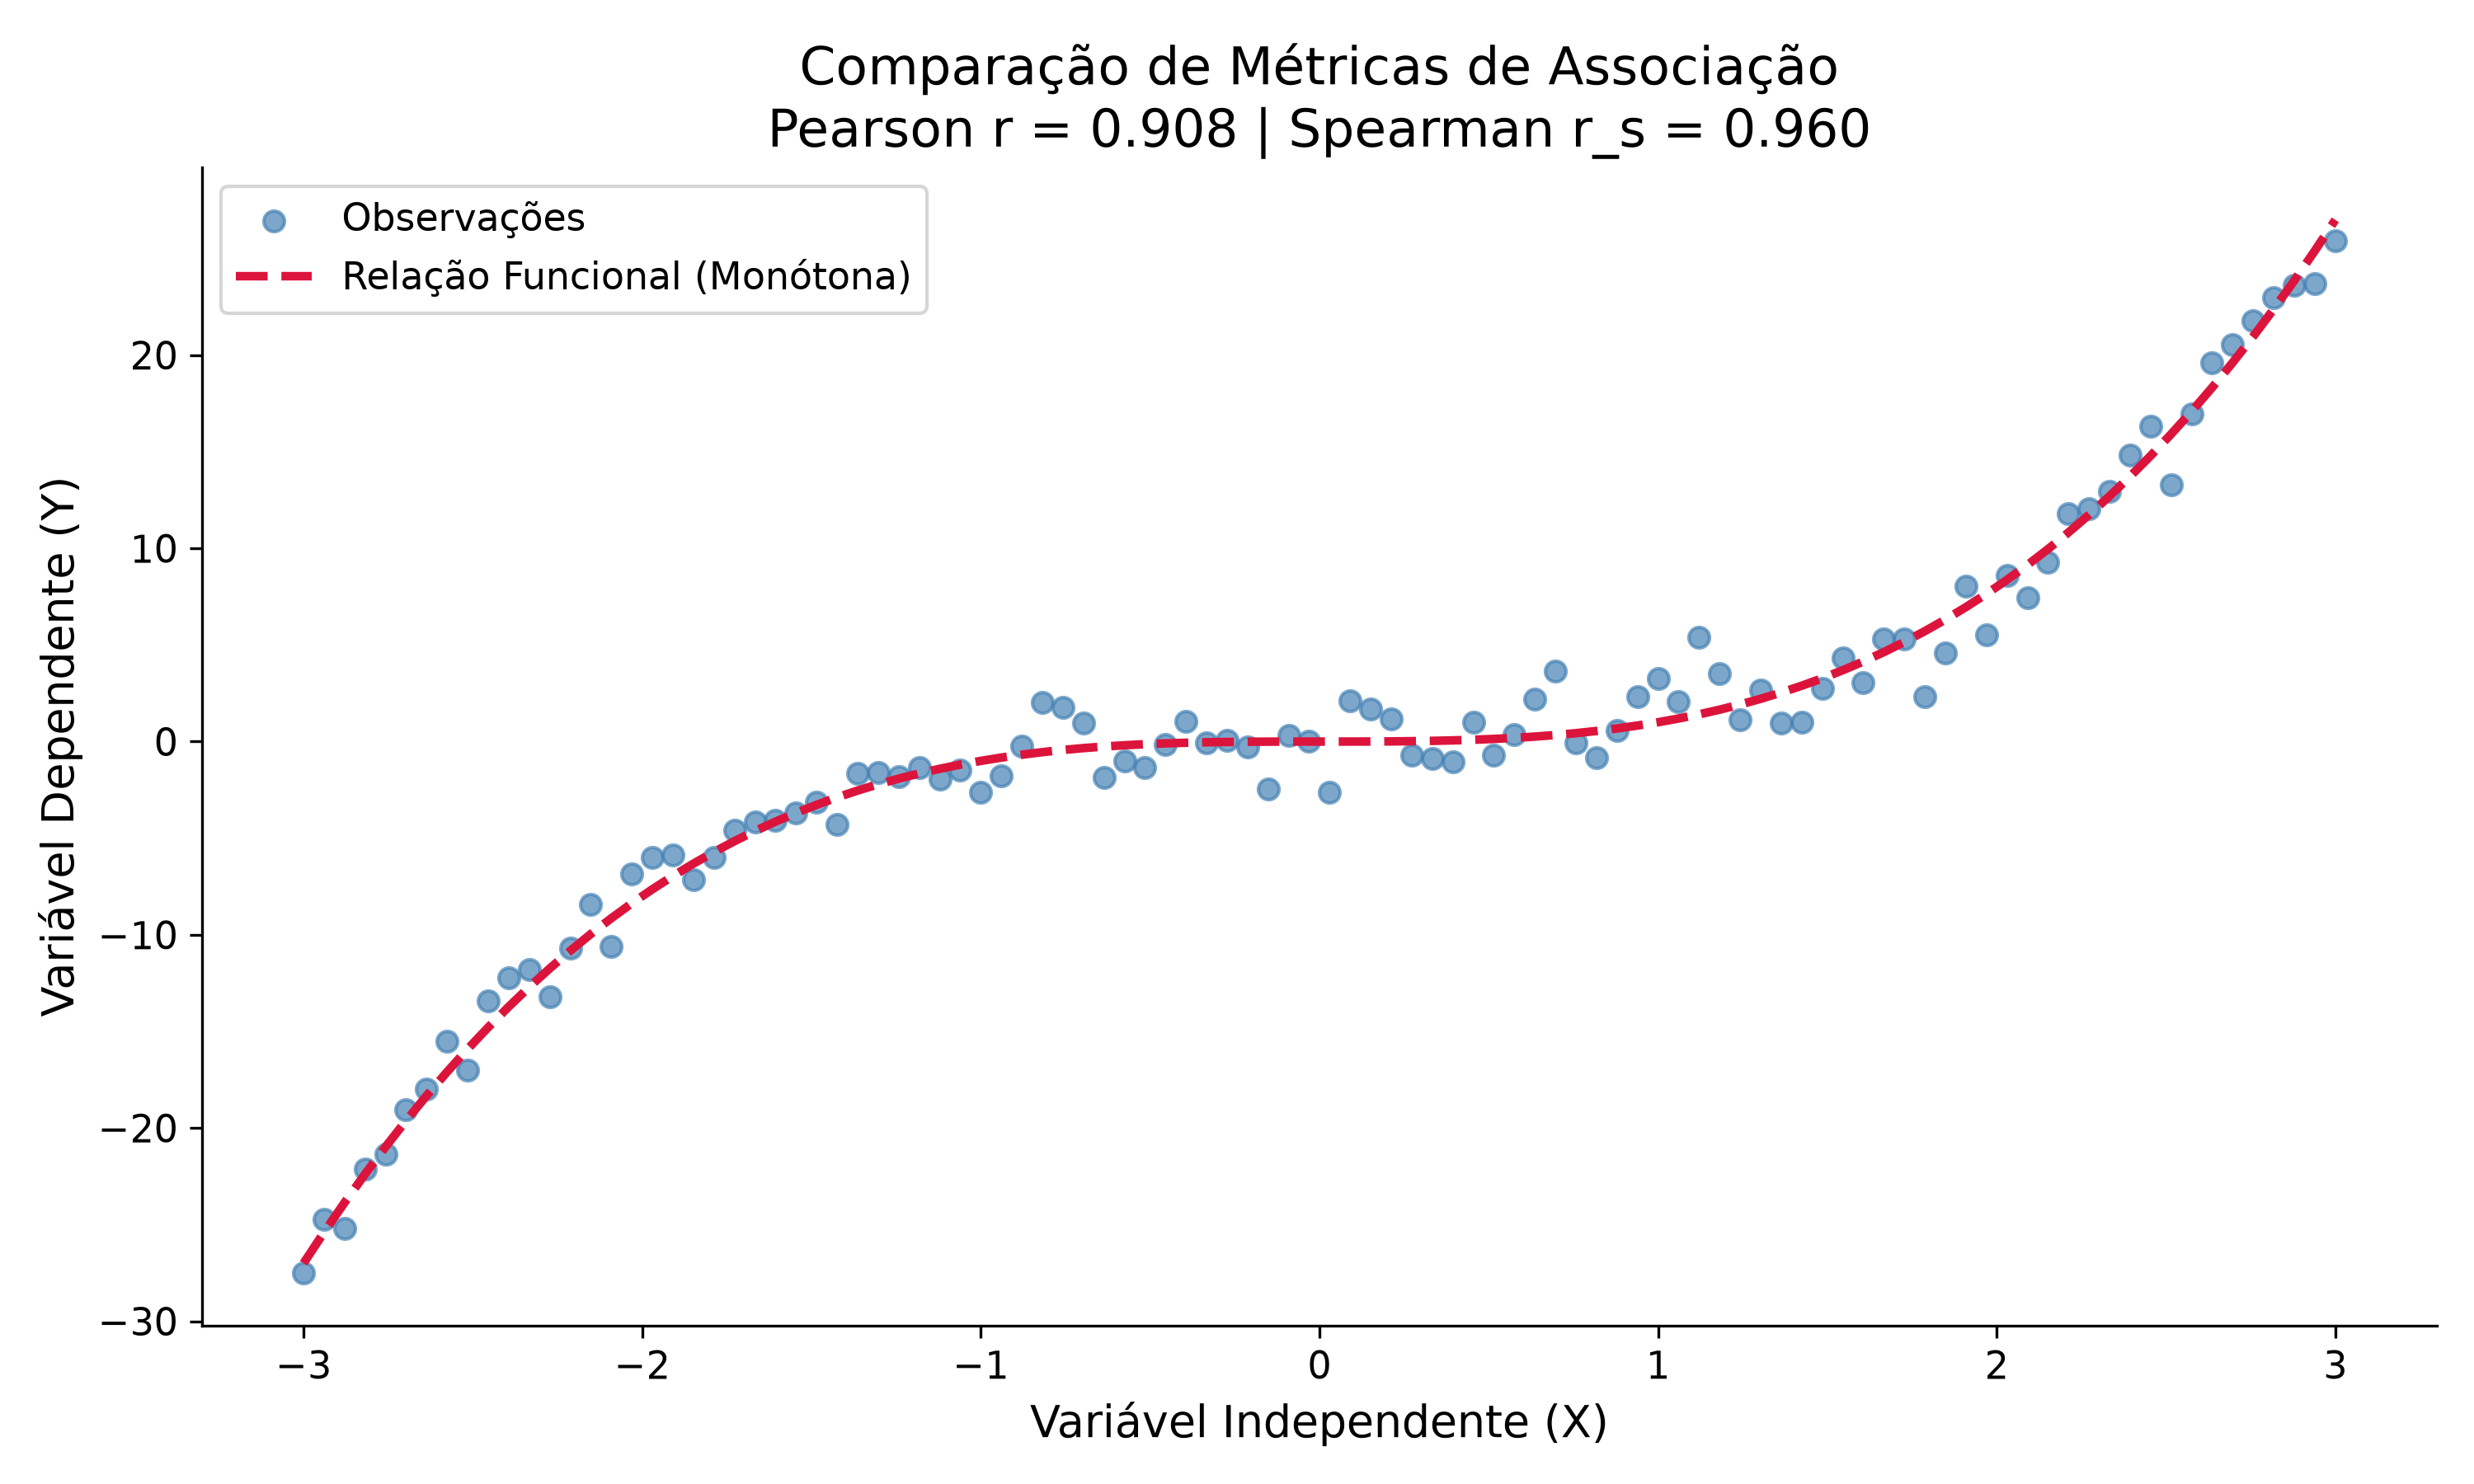
\includegraphics[width=0.88\textwidth]{grafico_pearson_vs_spearman.png}
        \end{column}
        \begin{column}{0.52\textwidth}
\begin{lstlisting}
# Codigo Python para comparar
from scipy import stats
import numpy as np

# Gerar dados exponenciais
x = np.linspace(1, 10, 50)
y = np.exp(x) + np.random.normal(0, 500, size=50)

# Calcular coeficientes
r_p, _ = stats.pearsonr(x, y)
r_s, _ = stats.spearmanr(x, y)

print(f"Pearson: {r_p:.4f}")
print(f"Spearman: {r_s:.4f}")
\end{lstlisting}
        \end{column}
    \end{columns}
\end{frame}

\begin{frame}{O Paradoxo de Simpson}
    \begin{itemize}
        \item Fenômeno no qual uma associação de dados observada em múltiplos subgrupos de forma consistente se \textbf{inverte} ou \textbf{desaparece} quando os dados são combinados no agregado.
        \item Ocorre por ignorar variáveis de confusão importantes que controlam os dados (ex: idade, demografia, fatores temporais).
        \item \textbf{Implicação para Tomada de Decisão:}
        \begin{itemize}
            \item Confiar cegamente em estatísticas globais agregadas pode levar a inferências completamente equivocadas sobre a realidade física.
        \end{itemize}
    \end{itemize}
\end{frame}

\begin{frame}{Estudo de Caso 1: Colesterol vs. Exercício (Agregado)}
    \begin{columns}
        \begin{column}{0.5\textwidth}
            \textbf{Aparência Enganosa:}
            \begin{itemize}
                \item No agregado geral (todos os dados combinados), a correlação entre exercício e colesterol é positiva ($r \approx 0.35$).
                \item Isso parece indicar que se exercitar mais aumenta o colesterol!
                \item \textbf{Explicação:} Trata-se de uma associação espúria causada pela omissão de uma variável de confusão (idade).
            \end{itemize}
        \end{column}
        \begin{column}{0.5\textwidth}
            \centering
            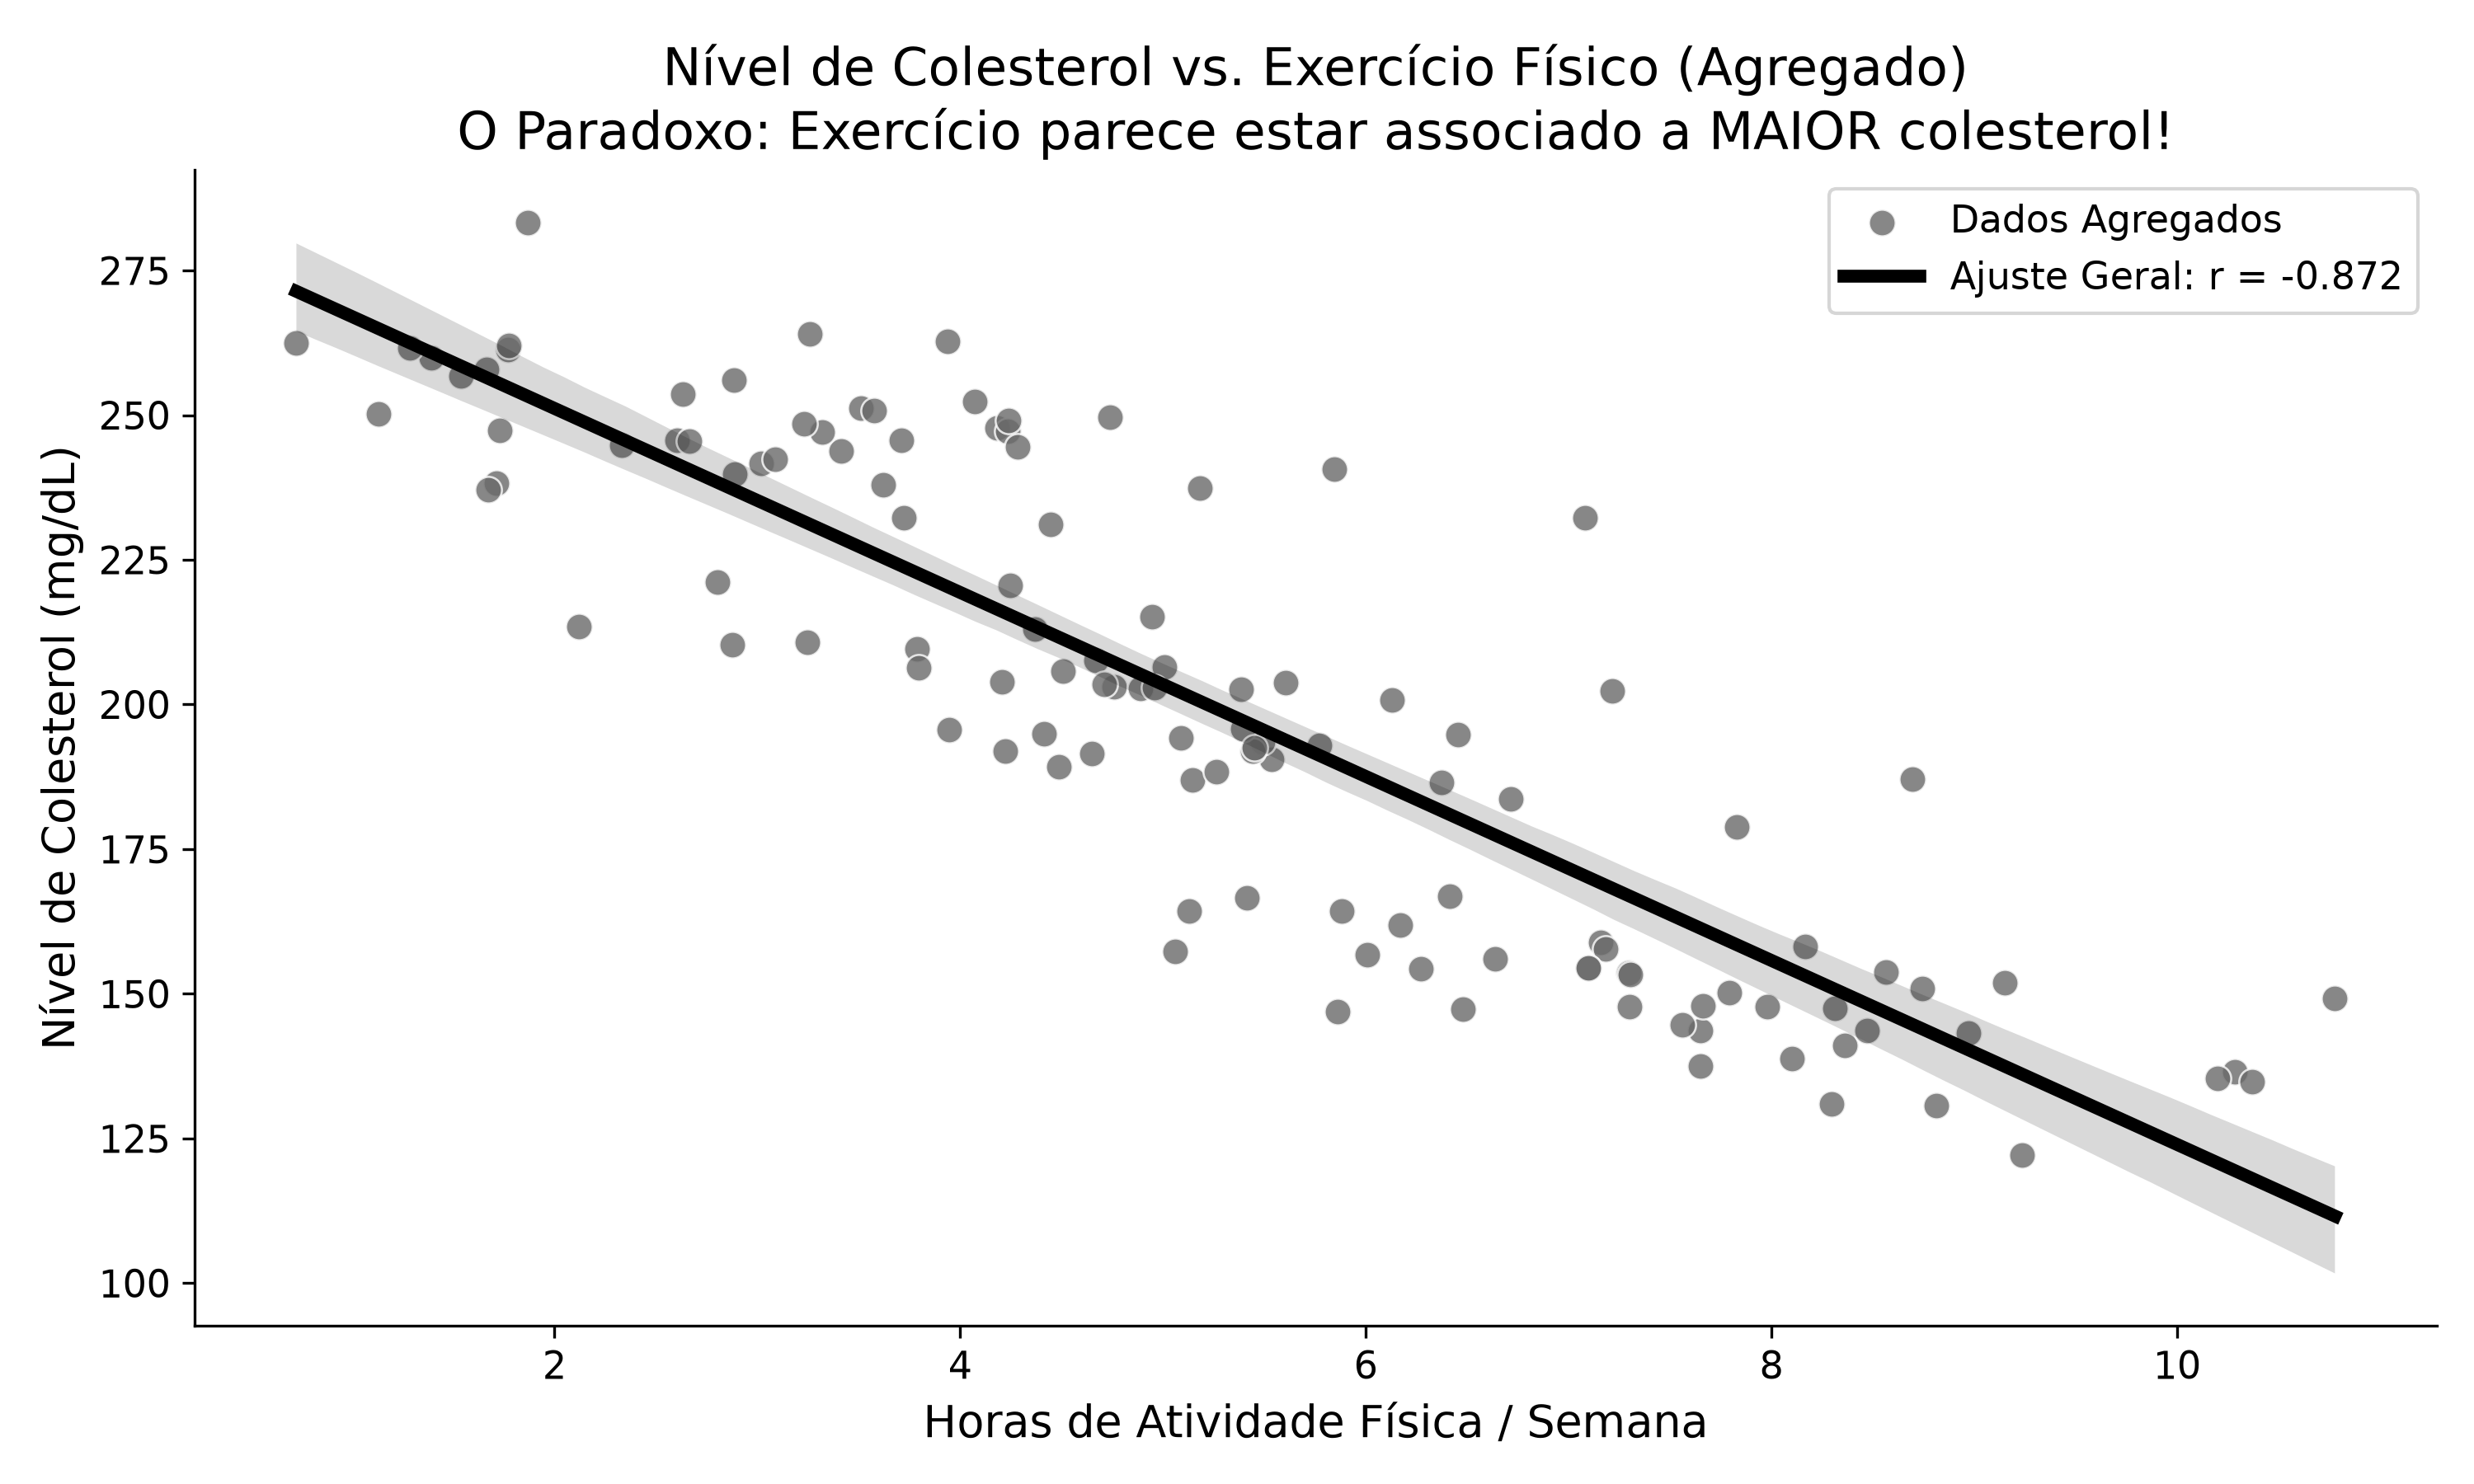
\includegraphics[width=0.95\textwidth]{simpson_agregado.png}
        \end{column}
    \end{columns}
\end{frame}

\begin{frame}{Estudo de Caso 1: Colesterol vs. Exercício (Estratificado)}
    \begin{columns}
        \begin{column}{0.5\textwidth}
            \textbf{A Estratificação Revela:}
            \begin{itemize}
                \item Ao agrupar por idade, descobrimos que em todas as faixas (Jovens, Adultos e Idosos) a correlação é negativa ($r \approx -0.58$).
                \item Pessoas idosas têm colesterol maior e se exercitam menos, o que distorce a análise agregada geral.
                \item A tomada de decisão correta exige a análise estratificada.
            \end{itemize}
        \end{column}
        \begin{column}{0.5\textwidth}
            \centering
            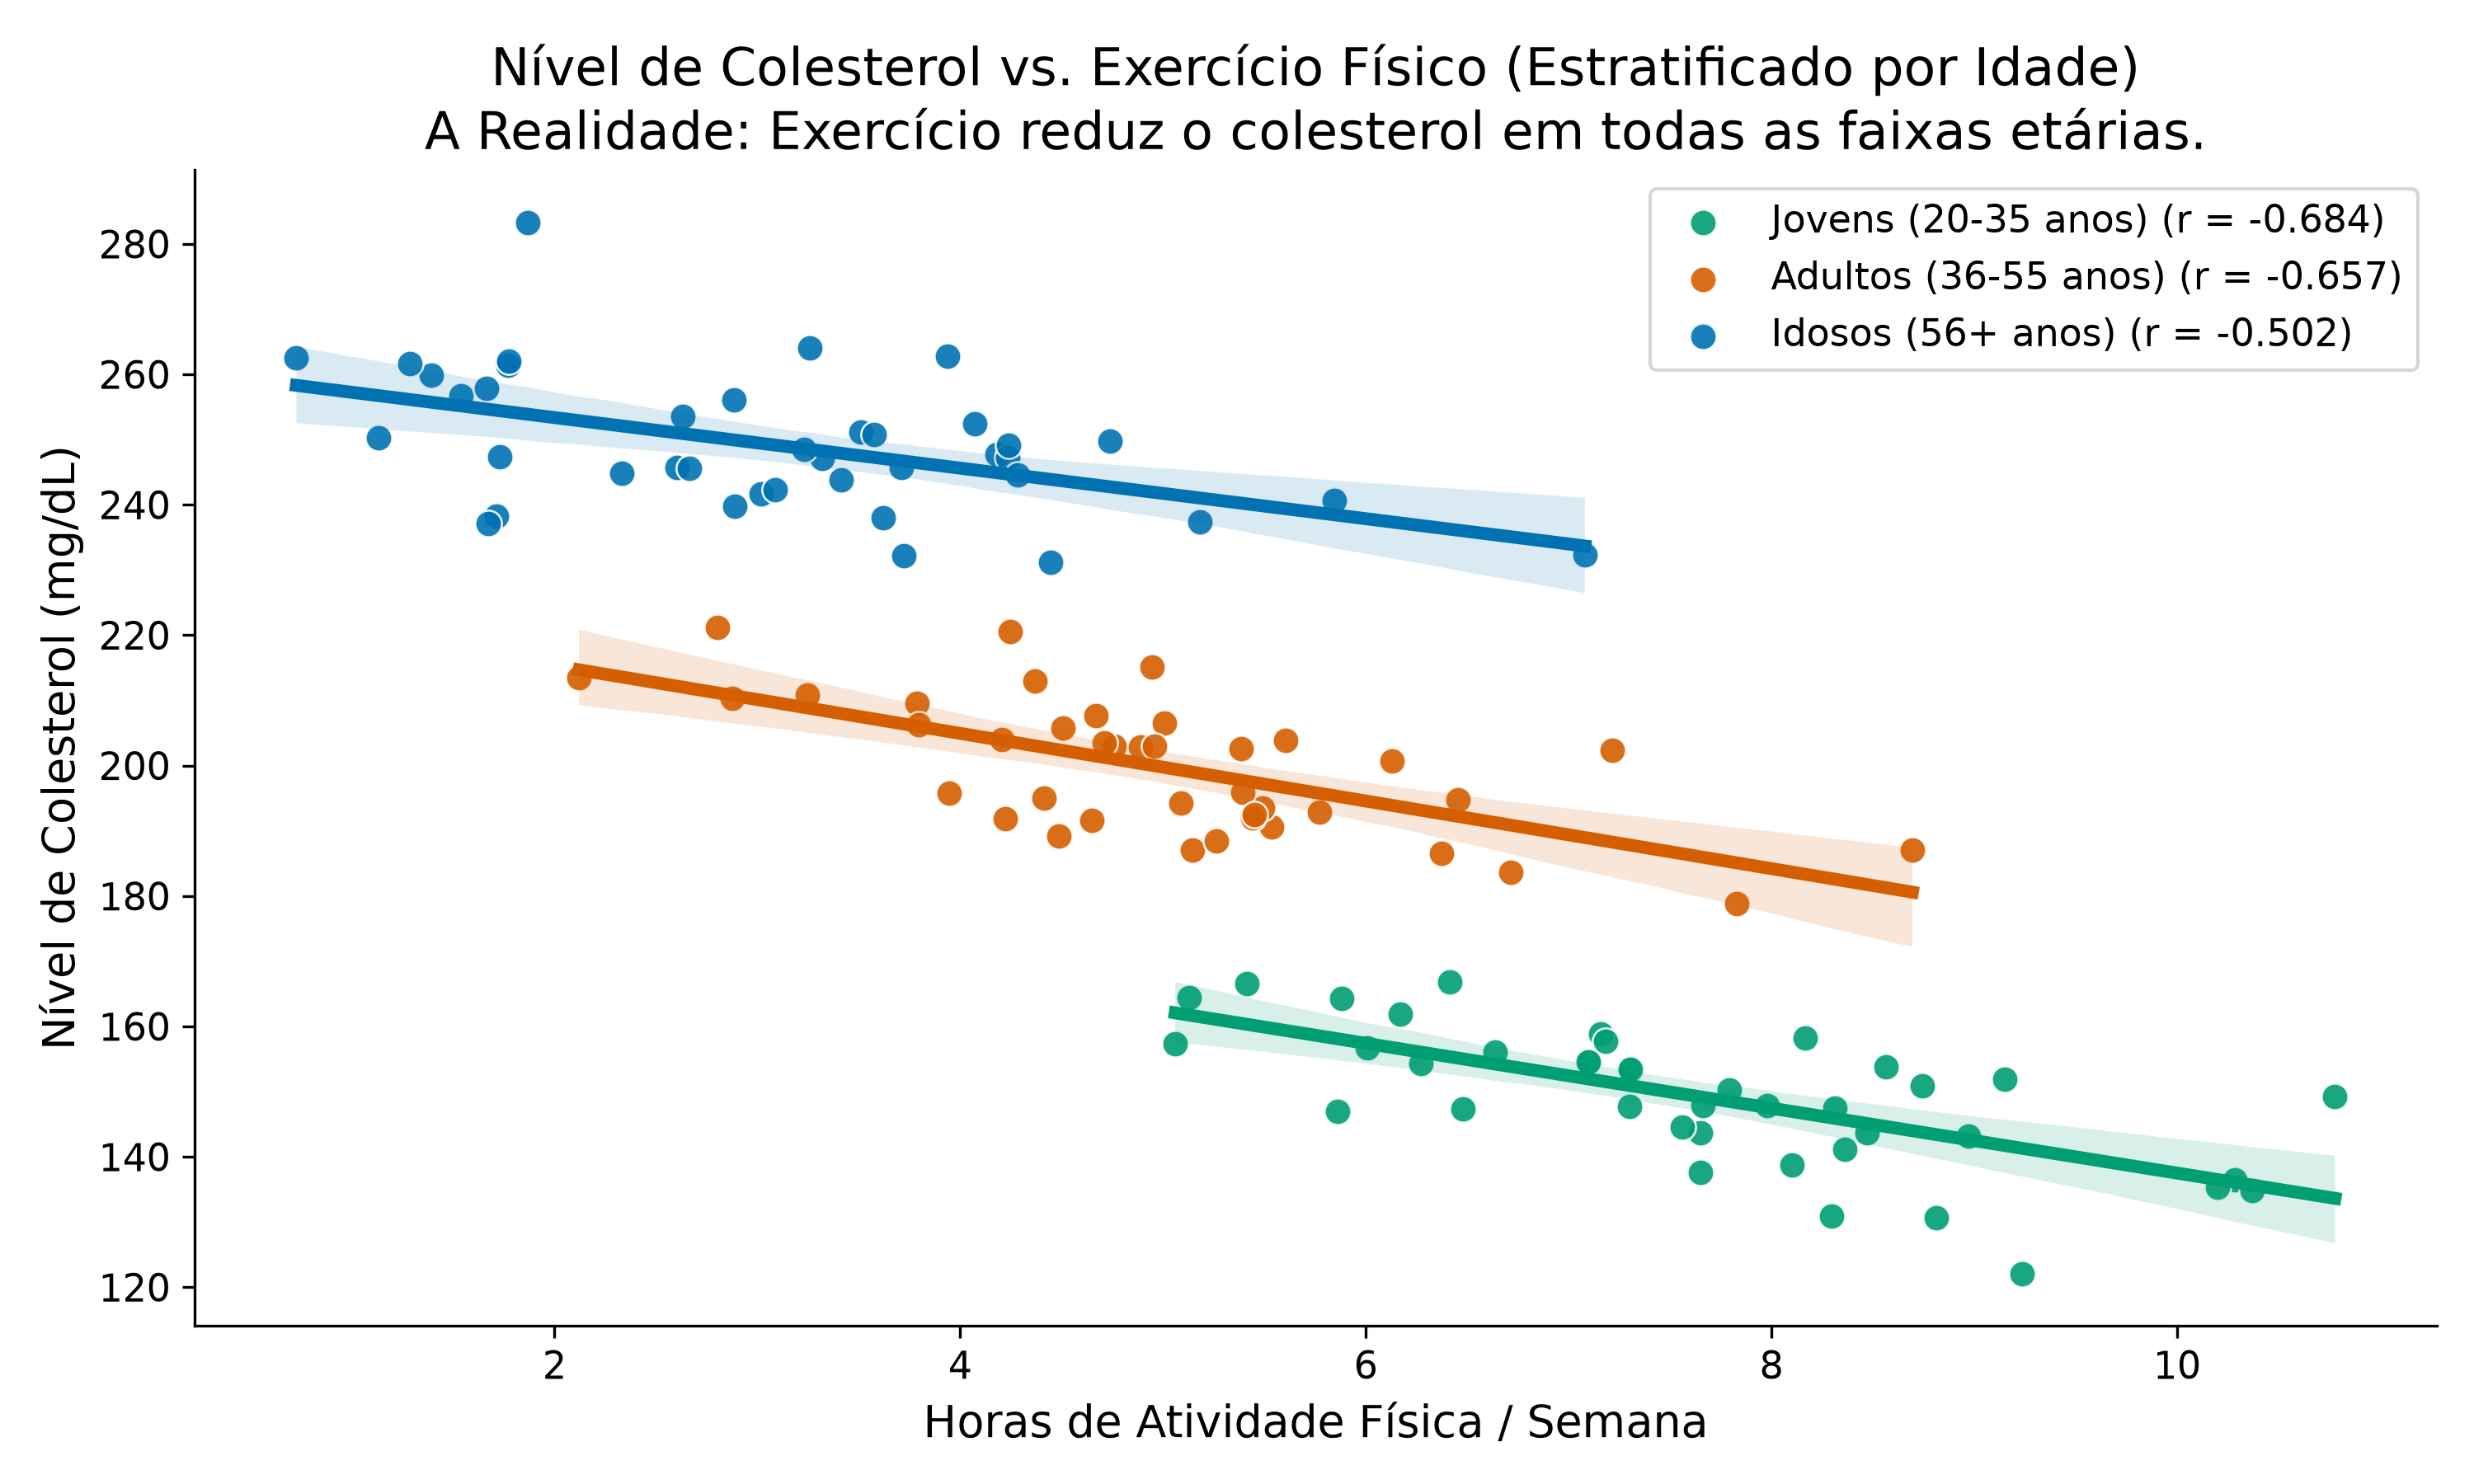
\includegraphics[width=0.95\textwidth]{simpson_estratificado.png}
        \end{column}
    \end{columns}
\end{frame}

\begin{frame}{Estudo de Caso 2: Taxa de Letalidade de COVID-19}
    \begin{itemize}
        \item Em dados da fase inicial da pandemia de COVID-19:
        \begin{itemize}
            \item A taxa de letalidade agregada da Itália era significativamente superior à da China.
            \item \textbf{Paradoxo:} Ao comparar as taxas segregadas por faixas etárias individuais (ex: 20-29, 30-39, etc.), a taxa chinesa era superior ou igual em praticamente todas as faixas!
        \end{itemize}
        \item \textbf{Por que isso ocorreu?}
        \begin{itemize}
            \item A Itália possui uma proporção muito maior de idosos em sua demografia comparada à China.
            \item Como os idosos são mais vulneráveis ao vírus, o grande número de casos em idosos na Itália inflou o indicador geral agregado do país, ocultando a menor taxa interna de letalidade específica por faixa etária.
        \end{itemize}
    \end{itemize}
\end{frame}

\begin{frame}{Associação não é Causalidade}
    \begin{itemize}
        \item Uma correlação linear robusta entre duas variáveis quantitativas ($r \approx 0.95$) descreve apenas a força de seu comportamento linear conjunto.
        \item \textbf{NÃO} comprova que a variação de $X$ causa diretamente a variação de $Y$.
        \item Exemplos clássicos de correlações espúrias (coincidência temporal):
        \begin{itemize}
            \item Gasto dos EUA em ciência vs. suicídios por enforcamento.
            \item Consumo de queijo por pessoa vs. mortes por se enrolar em lençóis.
        \end{itemize}
        \item \textbf{Regra de Ouro:} Use a correlação para formular hipóteses, mas recorra a experimentos controlados ou análise de variáveis de confusão para estabelecer causalidade.
    \end{itemize}
\end{frame}
